
%(BEGIN_QUESTION)
% Copyright 2010, Tony R. Kuphaldt, released under the Creative Commons Attribution License (v 1.0)
% This means you may do almost anything with this work of mine, so long as you give me proper credit

The energy stored in an archer's bow when fully drawn is equal to the amount of mechanical work invested by the archer in drawing the string back.  This potential energy is the integral of force ($F$) over increments of distance ($dx$) over an interval of distance beginning at $x_0$ and finishing at $x_f$:

$$E_p = \int_{x_0}^{x_f} F \> dx$$

Approximately calculate the amount of energy stored in a compound bow drawn to 30 inches, given the following force-draw curve:

$$\includegraphics[width=15.5cm]{i04281x01.eps}$$

Express your answer in units of {\it foot-pounds}.

\vskip 20pt \vbox{\hrule \hbox{\strut \vrule{} {\bf Suggestions for Socratic discussion} \vrule} \hrule}

\begin{itemize}
\item{} What is most important when solving problems such as this is to be able to explain {\it why} (not just {\it how}) to arrive at the correct value.  Try explaining the process of integration in your own words, as it applies to this particular problem.
\item{} How does the amount of work done between 10 and 15 inches of draw compare with the amount of work done between 25 and 30 inches of draw?
\end{itemize}

\underbar{file i04281}
%(END_QUESTION)





%(BEGIN_ANSWER)

$$E_p \approx 57.17 \hbox{ ft} \cdot \hbox{lb}$$

%(END_ANSWER)





%(BEGIN_NOTES)

$$\includegraphics[width=15.5cm]{i04281x02.eps}$$

$$E_p = \int_{10}^{30} F \> dx$$

$$E_p \approx 57.17 \hbox{ ft} \cdot \hbox{lb}$$

No single triangle or rectangle can properly emulate the shape of the area contained by the force-draw curve, so a series of triangles and rectangles were used here to approximate it.  The total energy represented by this sum of shape areas is 686 inch-pounds of energy.  Converting this into foot-pounds yields an answer of 57.17 ft-lbs.

%INDEX% Mathematics, calculus: integral (work)
%INDEX% Mathematics, calculus: integration (numerical)

%(END_NOTES)


